\chapter{Early warning, change points and fault typing}
\label{ch:more}

These three pieces sit on top of the main pipeline. They do \emph{not} change what is detected or how it is ranked (with one exception noted below). They add information for the operator.

\section{Early warning: a trend before the alarm}
\begin{simplebox}
Some faults arrive slowly. A memory leak climbs for ten minutes before the service dies. A normal alarm only fires when the line is crossed. An early warning looks at the \emph{direction} the number is heading. If a service's deviation has been rising steadily over the last two minutes, and the straight line through those points will cross the alarm line within the next two minutes, we flag it early.
\end{simplebox}

\begin{techbox}
For each rising-only feature, a least-squares line fitted to the load-aware residual $z$ over the last two minutes (24 readings) and projected two minutes ahead flags a service that has not reached the alarm level but will. Only lines with $R^2\ge0.6$ count, so a noisy up-down wobble does not trigger a warning.
\end{techbox}

\begin{figure}[H]
\centering
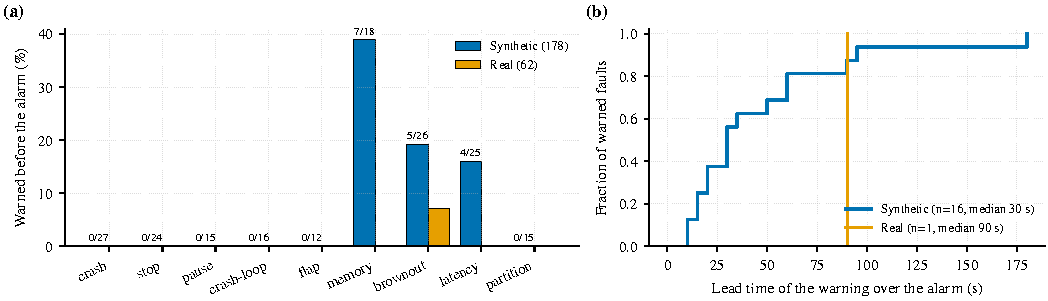
\includegraphics[width=0.98\textwidth]{fig_early.pdf}
\caption{Early warning. (a) Share of faults warned before the alarm, by fault class. (b) Lead time of the warnings over the alarm.}
\end{figure}

\begin{warnbox}
This is the \textbf{weakest} part of the system, and the report says so. On the synthetic set it warns before the alarm for 13 of 178 faults (7 of 18 memory leaks, 4 of 25 latency faults, 2 of 26 brownouts) with a median lead of 25 seconds and 0.8 false warning episodes per fault-free hour. On the real systems it fired before the alarm for \emph{none} of the 62 faults, because those faults are abrupt, and raised 6.9 false warning episodes per hour. If asked ``does it predict failures?'', say ``it warns early for some gradual faults in simulation; on our real, abrupt faults it did not, and we report it as the weakest component''.
\end{warnbox}

\section{Change-point alarms: faster, at a price}
\begin{simplebox}
A usual alarm waits until a number is clearly beyond its normal range. A \emph{change-point} detector instead notices that the \emph{average has shifted}, which can happen a few seconds sooner. It is like noticing that a car has started drifting before it actually leaves the lane. The trade is that it also reacts to harmless shifts, so you spend more time in alarm.
\end{simplebox}

\begin{techbox}
We used online Page--Hinkley change-point detection on the raw metrics as an additional alarm source. On the real systems it lifts the detected fraction from 90\% to 95\% and cuts the median detection delay from 11.3\,s to 4.8\,s, but alarm time rises from 8\% to 16\%. On the synthetic set, whose faults are abrupt, the curves almost coincide. It is available as a research variant; the shipped default does not use it.
\end{techbox}

\begin{figure}[H]
\centering
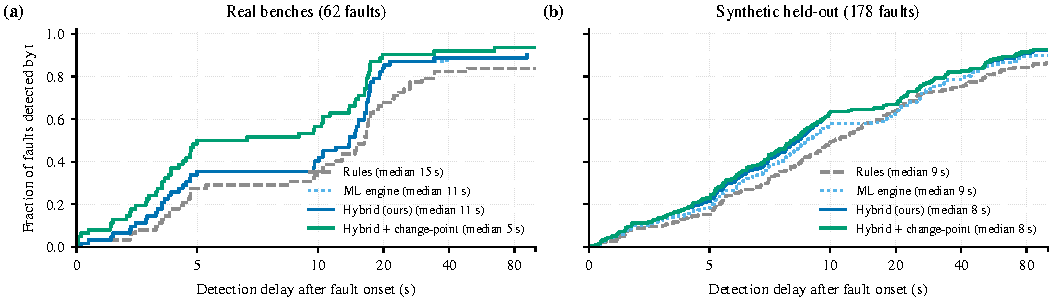
\includegraphics[width=0.98\textwidth]{fig_delay.pdf}
\caption{Detection delay after fault onset as a cumulative distribution.}
\end{figure}

\begin{saybox}
``Change-point alarms cut the median detection delay from 11.3 to 4.8 seconds on the real systems, but they double the time in alarm, from 8 to 16 percent. We list it as a trade-off, not a free win, which is why it is not the default.''
\end{saybox}

\section{Naming the type of fault and attaching a runbook}
\begin{simplebox}
When an alarm fires and we have a top suspect, the engineer's next question is ``what kind of problem is it?'': did it crash, was it stopped on purpose, is it crash-looping, is it leaking memory, is it just slow? We use a small decision-tree-style classifier (a random forest) that looks at 35 things about that service's recent telemetry and names the type. Then we attach a short checklist of two to four concrete commands for that type, like ``check \code{docker logs}'' or ``look at the memory limit''. The classifier only labels and advises. It never changes the alarm or the ranking.
\end{simplebox}

\begin{techbox}
At the alarm, 35 features of the top suspect's telemetry (container-state history, exit code, number of separate outages, memory slope, CPU and throttling change, latency and error ratios against a pre-fault baseline, network drop, number of anomalous callers) go to a random forest that names the fault type: crash, stop, pause, crash-loop, flap, memory, brownout, latency or partition. A runbook of two to four concrete checks per type is attached. With the true service the forest is correct for 99\% of synthetic faults 60\,s after the alarm; on the engine's own suspect it is 79\%, because a wrong suspect is rarely typed correctly. On the real systems a hand-written decision list generalises best (64\% on the suspect, 84\% on the true service), because real flaps are pause cycles and real brownouts on idle services show no throttling --- differences between the simulator and reality that the learned models absorb as synthetic-specific patterns.
\end{techbox}

\begin{figure}[H]
\centering
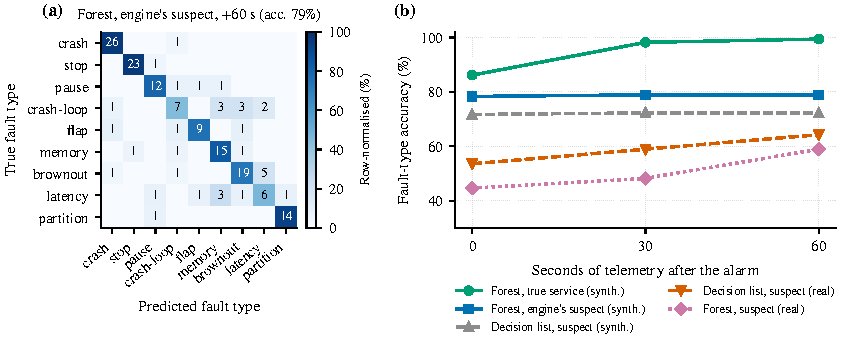
\includegraphics[width=0.78\textwidth]{fig_diag.pdf}
\caption{Fault-type diagnosis. (a) Confusion matrix of the random forest on the engine's suspect 60\,s after the alarm. (b) Accuracy against seconds of telemetry after the alarm.}
\end{figure}

\section{Learned directions: a robustness feature}
\begin{figure}[H]
\centering
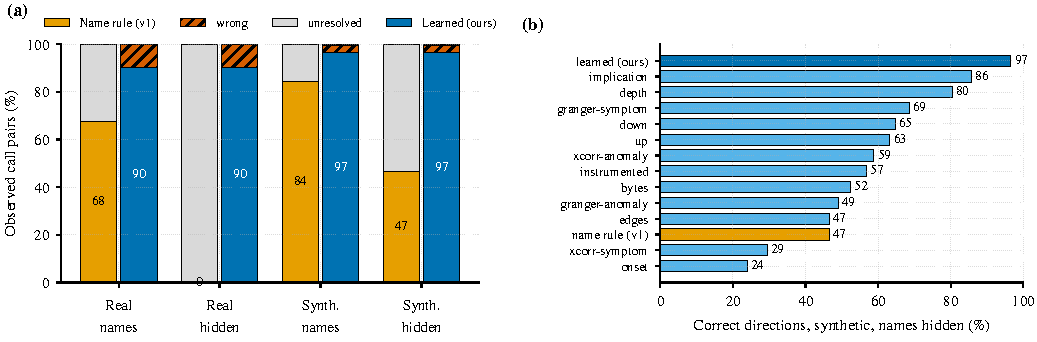
\includegraphics[width=0.98\textwidth]{fig_dirs.pdf}
\caption{Call directions. (a) Share of observed true-call pairs oriented correctly, wrongly or left unresolved, with names shown or hidden. (b) Correct share of each signal with names hidden.}
\end{figure}

\begin{simplebox}
We explained learned directions in Part~\ref{ch:graph}. Here is the result in plain words. When names tell you which service is a database, which is a gateway and so on, the simple name rule gets 21 of 31 pairs right and leaves 10 undecided; the learned rule gets 27 of 31 (4 wrong). When names are hidden (renamed ``alpha, bravo, ...''), the name rule is undecided for every pair and the learned rule is unchanged. On ranking the effect is small: with names available, learned directions are \emph{not} better than the name rule (68\% against 71\%, $-3.2$ points, not significant). With names hidden they reach 68\% against 66\% for the name rule and 71\% for the true graph. So learned directions are a \emph{robustness} mechanism, not an accuracy gain.
\end{simplebox}

\section{Cost: can this run live?}
\begin{figure}[H]
\centering
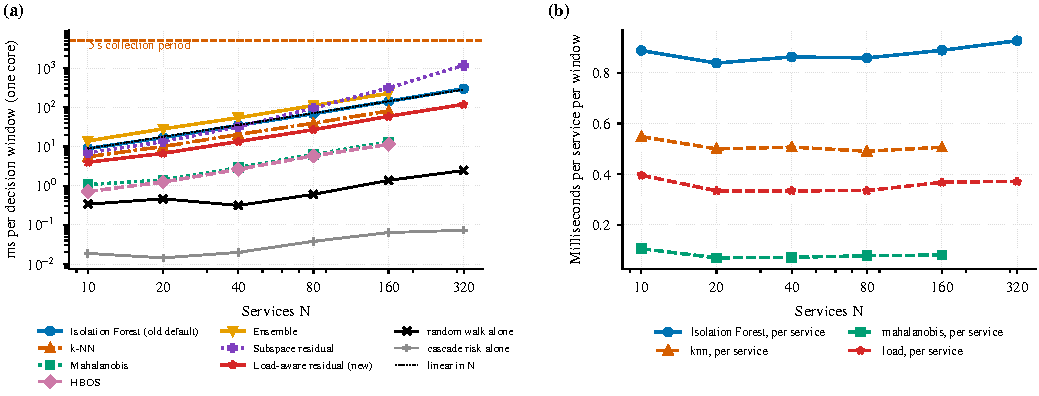
\includegraphics[width=0.98\textwidth]{fig_scale.pdf}
\caption{Cost of one decision window against the number of services (single core, logarithmic axes; the dashed line is the 5\,s collection period).}
\end{figure}

\begin{simplebox}
Does the thinking take long? No. For one service, one decision takes about a third of a millisecond. For ten services about four milliseconds; for 320 services about a tenth of a second. The mapper only needs to finish within five seconds, so it has a lot of room. The cost grows in a straight line with the number of services: twice the services, twice the cost.
\end{simplebox}

\begin{techbox}
The adopted load-aware model costs about $0.37$\,ms per service per window and grows linearly: 4.0\,ms for 10 services, 26.8\,ms for 80 and 119\,ms for 320 (95th percentile 356\,ms), always far below the 5\,s collection period. The old forest cost about $0.9$\,ms per service (296\,ms for 320) with 95th-percentile windows nine times the mean, because every service refits at once every ten readings; the load-aware model refreshes its baselines every four readings with a much smaller peak (about three times the mean). The subspace residual grows faster than linearly (1.2\,s for 320 services, with 11\,s windows at the 95th percentile) because its covariance has one row per service-signal pair. On the two benches (12 and 13 services) a window takes about 5\,ms. These are wall-clock times on one core of a shared four-core virtual machine, not a tuned benchmark.
\end{techbox}
